\chapter{Results} \label{results}
%\begin{figure}[H]
%\centering
%    \begin{minipage}{0.45\textwidth}
%%        \centering
%        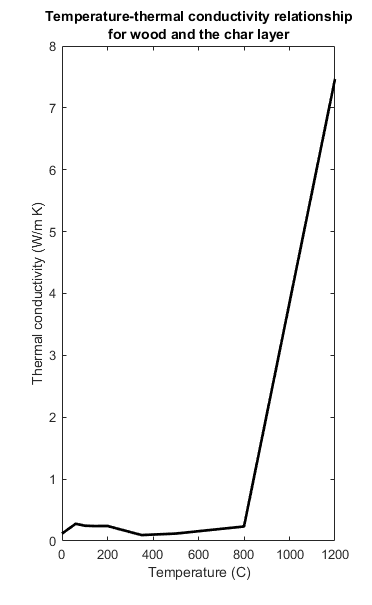
\includegraphics[width=0.9\textwidth]{figures/resultsk_cropped.png} % first figure itself
%        \caption{The resulting $\kappa$-values }
%        \label{kresult_fig}
%    \end{minipage}
%    \begin{minipage}{0.45\textwidth}
%%        \centering
%        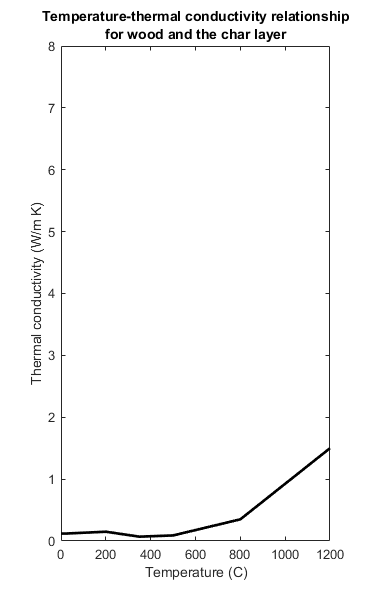
\includegraphics[width=0.9\textwidth]{figures/eurok_samescale_cropped.png} % second figure itself
%        \caption{The original $\kappa$-values}
%        \label{scalekeuro_fig}
%    \end{minipage}
%\end{figure}\

The results of the MCMC analysis as well as the MAP optimization is visualised in the section below.
\section{Resulting k-values}

The thermal conductivity ($\kappa$-values) at key temperatures was the main goal of this project. 
As can be seen in Figure \ref{kresult_euro_fig} there was quite a drastic difference in the thermal diffusivity at 1200 \textdegree C and between 0\textdegree C and 200\textdegree C.
The large difference at 1200\textdegree C is due to how the model is created, at that temperature the majority of the heat is transferred through thermal radiation.
The model did not model thermal radiation separately but instead incorporated the radiation into a equivalent conduction.
Between 0\textdegree C and 200\textdegree C the modelling of the evaporation was moderately succesful as a spike can be seen at 100 \textdegree C.  
\begin{figure}[H]
\centering
	\label{kresult_euro_fig}
	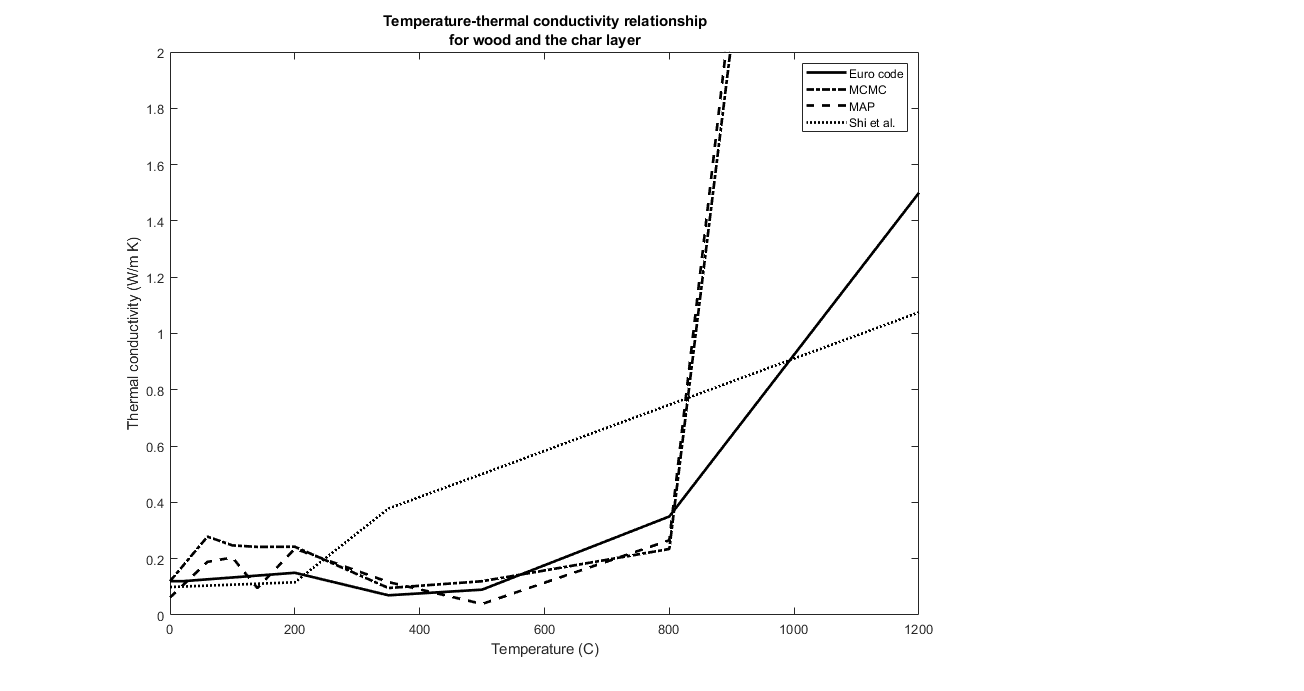
\includegraphics[width=\textwidth]{figures/kvalues_all_shi.png}
	\caption{Resulting $\kappa$ values compared to Euro-code standard values}
\end{figure}
 
 
 
\begin{figure}[b]
\label{histofig}
\centering
	\begin{subfigure}{}
	\centering
	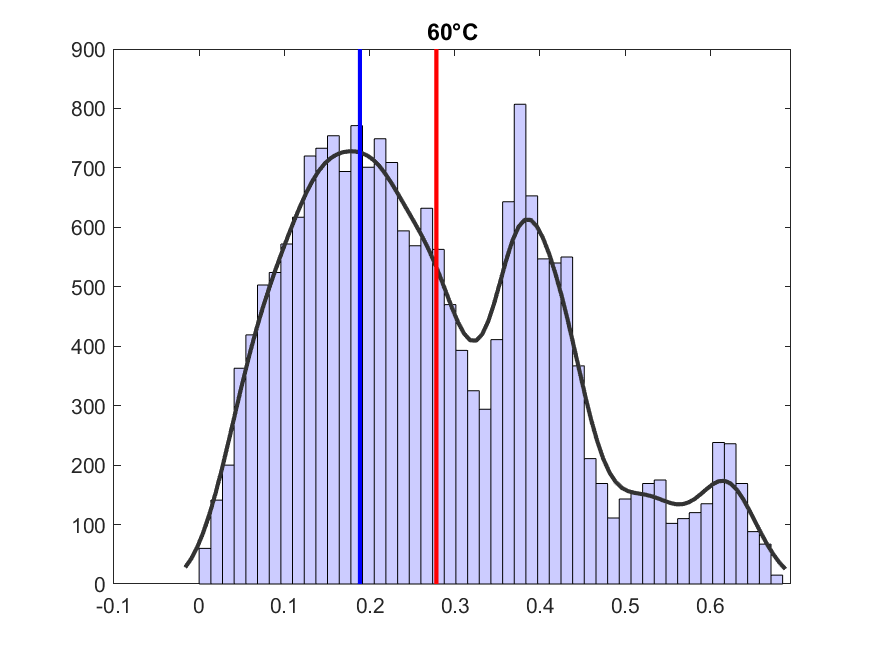
\includegraphics[width = 0.45\linewidth]{figures/histograph/histo1.png}
	\end{subfigure}
	\begin{subfigure}{}
	\centering
	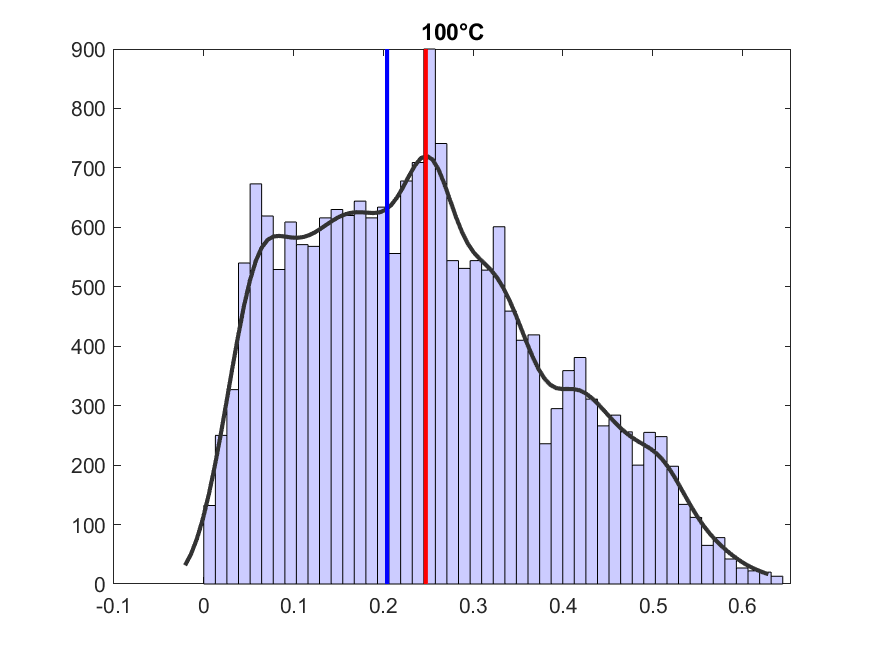
\includegraphics[width = 0.45\linewidth]{figures/histograph/histo2.png}
	\end{subfigure}
	\begin{subfigure}{}
	\centering
	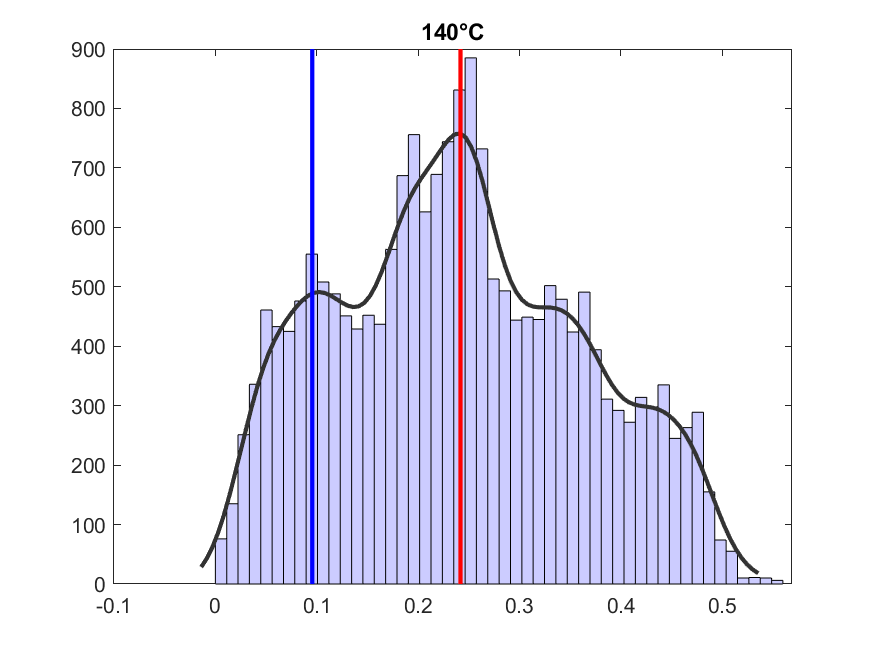
\includegraphics[width = 0.45\linewidth]{figures/histograph/histo3.png}
	\end{subfigure}
	\begin{subfigure}{}
	\centering
	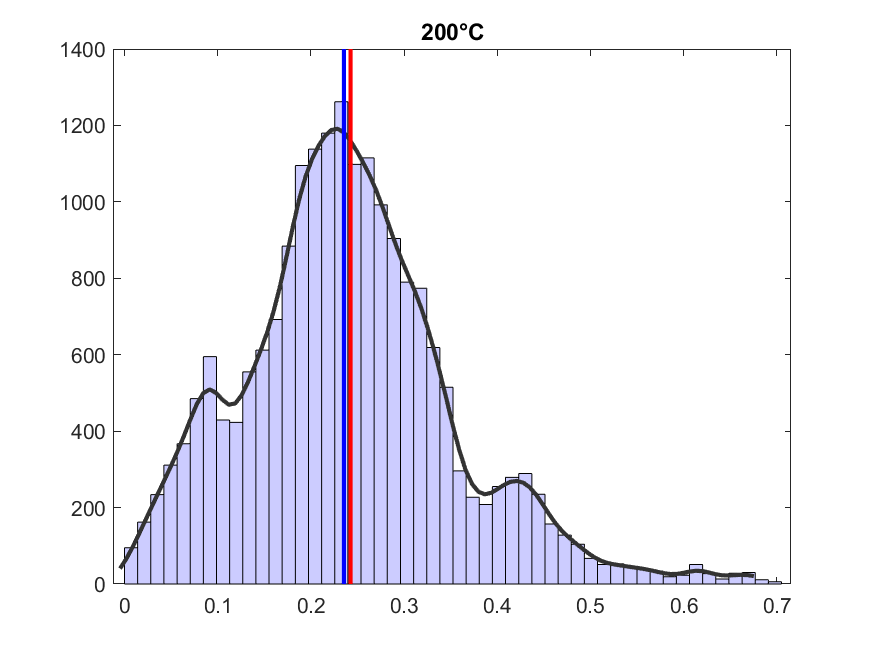
\includegraphics[width = 0.45\linewidth]{figures/histograph/histo4.png}
	\end{subfigure}
	\begin{subfigure}{}
	\centering
	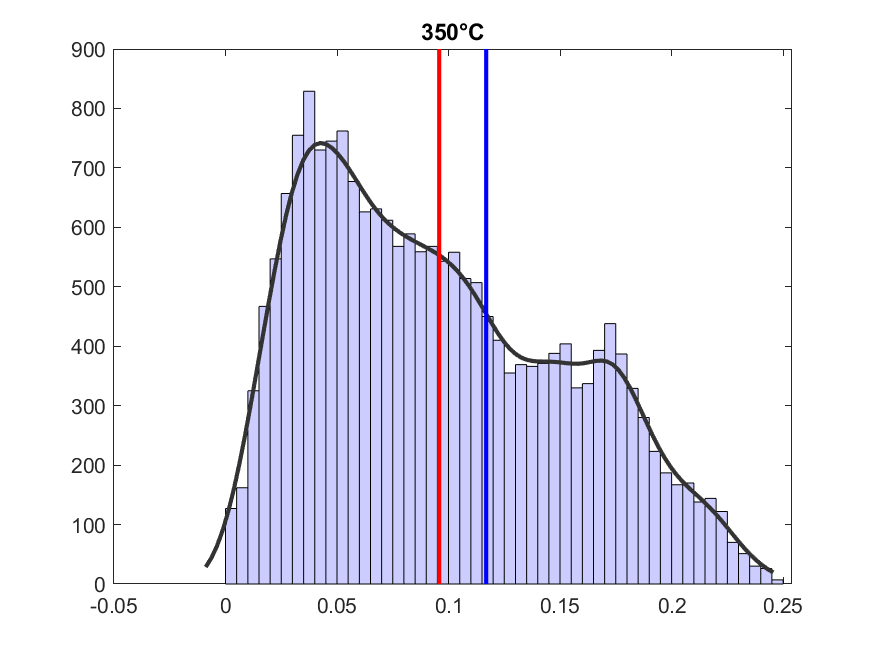
\includegraphics[width = 0.45\linewidth]{figures/histograph/histo5.png}
	\end{subfigure}
	\begin{subfigure}{}
	\centering
	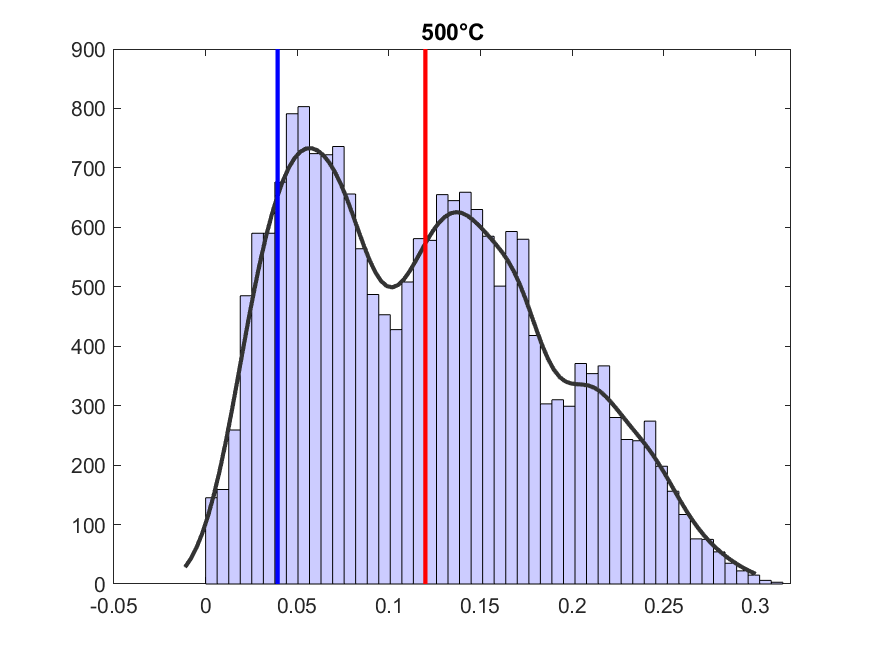
\includegraphics[width = 0.45\linewidth]{figures/histograph/histo6.png}
	\end{subfigure}
	\begin{subfigure}{}
	\centering
	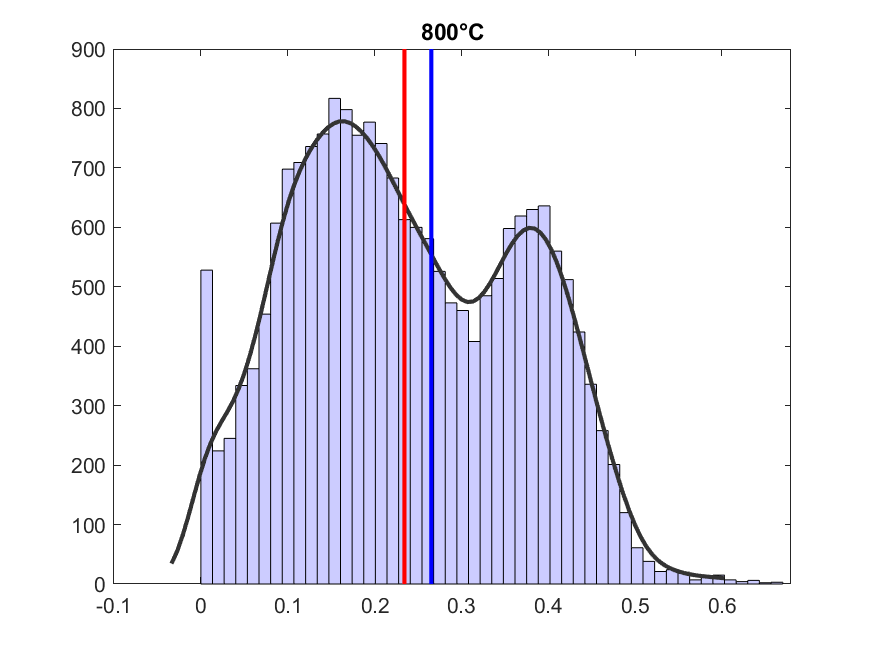
\includegraphics[width = 0.45\linewidth]{figures/histograph/histo7.png}
	\end{subfigure}
	\begin{subfigure}{}
	\centering
	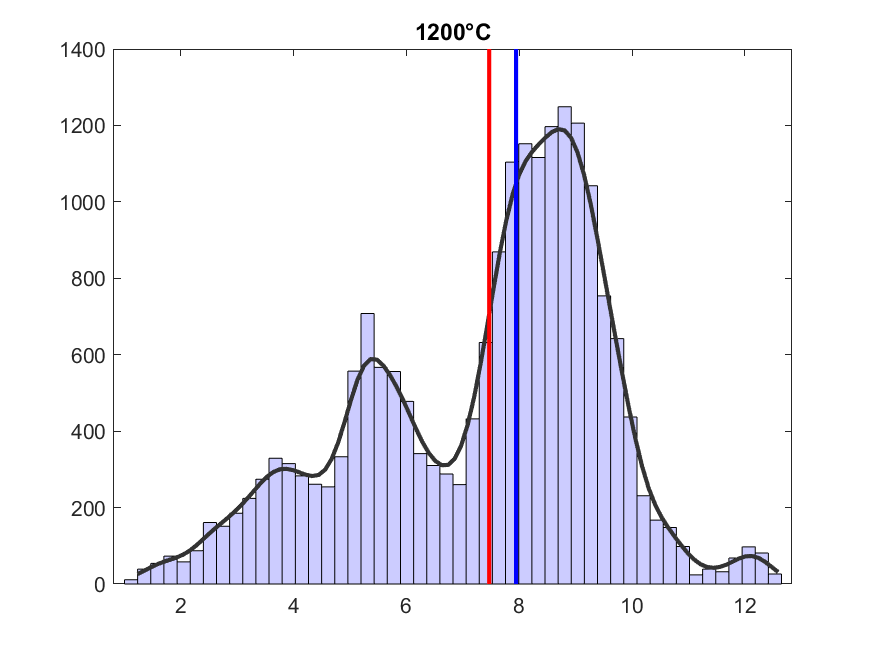
\includegraphics[width = 0.45\linewidth]{figures/histograph/histo8.png}
	\end{subfigure}
	\caption[short]{Histographs showing distribution at different temperatures}
\end{figure}


